% Compilation : pdflatex Dynamique_referentiels_non_galileens.tex (deux fois).
% Document autonome : texte, formules et figures TikZ modifiables.
% Les reperes Source renvoient aux pages du manuscrit.
\documentclass[11pt,a4paper]{article}
\usepackage[utf8]{inputenc}
\usepackage[T1]{fontenc}
\usepackage[provide=*,french]{babel}
\usepackage[scaled=.95]{helvet}
\renewcommand{\familydefault}{\sfdefault}
\usepackage{amsmath,amssymb,esint,array,tabularx}
\usepackage{geometry}
\geometry{left=15mm,right=15mm,top=18mm,bottom=18mm,headheight=14pt,headsep=6mm}
\usepackage{fancyhdr,lastpage,tikz}
\usetikzlibrary{arrows.meta,calc,decorations.pathreplacing,decorations.pathmorphing,decorations.markings,patterns}
\usepackage[most]{tcolorbox}
\usepackage{enumitem,titlesec,needspace,hyperref}
\hypersetup{hidelinks,pdftitle={Dynamique dans des référentiels non galiléens},pdfsubject={Cours de physique}}
\pagestyle{fancy}\fancyhf{}
\fancyhead[L]{\small Physique M3 - Dynamique en référentiel non galiléen - inspiré par les cours de Mme Mesnil}
\fancyhead[R]{\small\thepage/\pageref{LastPage}}
\fancyfoot[R]{\small PC-PC*}
\renewcommand{\headrulewidth}{0pt}
\setlength{\parindent}{0pt}\setlength{\parskip}{5pt}
\setlength{\abovedisplayskip}{7pt}\setlength{\belowdisplayskip}{7pt}
\setlist[itemize]{leftmargin=5mm,itemsep=3pt,topsep=3pt,label=\(\rightarrow\)}
\setlist[enumerate]{leftmargin=6mm,itemsep=3pt,topsep=3pt}
\renewcommand{\thesection}{\Roman{section}}
\renewcommand{\thesubsection}{\thesection.\arabic{subsection}}
\titleformat{\section}{\Large\bfseries}{\thesection.}{.4em}{}
\titleformat{\subsection}{\large\bfseries}{\thesubsection.}{.4em}{}[\titlerule]
\titleformat{\subsubsection}{\normalsize\bfseries}{\alph{subsubsection})}{.5em}{}
\titlespacing*{\section}{0pt}{11pt}{6pt}
\titlespacing*{\subsection}{0pt}{9pt}{5pt}
\titlespacing*{\subsubsection}{0pt}{8pt}{4pt}
\newtcolorbox{cadre}[1][]{enhanced,sharp corners,colback=white,colframe=black,boxrule=1.1pt,left=7pt,right=7pt,top=5pt,bottom=5pt,before skip=7pt,after skip=7pt,#1}
\newtcolorbox{exemple}[1][]{enhanced,sharp corners,colback=white,colframe=black,boxrule=.7pt,left=8pt,right=8pt,top=6pt,bottom=6pt,before skip=8pt,after skip=8pt,#1}
\tcbset{etoiles/.style={width=\dimexpr\linewidth-22mm\relax,overlay={\node[anchor=west,inner sep=0pt,font=\small] at ([xshift=2mm]frame.east) {\(#1\)};}}}
\newcommand{\dd}{\mathrm d}
\newcommand{\vv}{\vec v}
\newcommand{\grad}{\overrightarrow{\mathrm{grad}}}
\newcommand{\pd}[2]{\frac{\partial #1}{\partial #2}}
\newcommand{\ux}{\vec u_x}\newcommand{\uy}{\vec u_y}\newcommand{\uz}{\vec u_z}
\newcommand{\cste}{\mathrm{cste}}
\newcommand{\titr}[1]{\par\textbf{\underline{#1}}\par\nopagebreak[3]}
\newcommand{\planpart}[2]{\par\vspace{5pt}{\bfseries #1. #2}\par}
\newcommand{\plansub}[2]{\hspace*{7mm}{\itshape #1) #2}\par}
\newcommand{\plansubsub}[1]{\hspace*{15mm}{\itshape #1}\par}
\tikzset{>=Stealth,every node/.style={font=\small},flow/.style={thick,->},edge/.style={thick}}
\newcommand{\etoiles}[1]{\foreach \i in {1,...,#1}{\mathord{\star}\,}}
\newcommand{\R}{\mathcal R}\newcommand{\Rg}{\R_g}
\newcommand{\Om}{\vec\Omega_{\R'/\Rg}}
\newcommand{\Fie}{\vec F_{\mathrm{ie}}}\newcommand{\Fic}{\vec F_{\mathrm{ic}}}
\renewcommand{\ae}{\vec a_e}\newcommand{\ac}{\vec a_c}
\newcommand{\vp}{\vec v_{\R'}}\newcommand{\ap}{\vec a_{\R'}}
\newcommand{\ag}{\vec a_{\Rg}}\newcommand{\mt}{m_{\mathrm{tot}}}
\newcommand{\D}[2]{\left.\frac{\dd #1}{\dd t}\right|_{#2}}
\newcommand{\mom}[1]{\vec{\mathcal M}_{#1}}
\newcommand{\pow}{\mathcal P}\newcommand{\Ep}{E_{p\mathrm{ie}}}
\newcommand{\rep}[1]{\draw[->] (0,0)--(1.1,0);\draw[->] (0,0)--(0,1.2);\draw[->] (0,0)--(-.6,-.7);\node[below right] at (.3,-.2){$#1$};}
\newcommand{\frames}[1]{\begin{tikzpicture}[scale=.7]
\rep{\Rg}\node[above left] at (0,0){$O$};
\begin{scope}[shift={(4,.5)},rotate=40]\rep{}\end{scope}\node[right] at (4.8,.3){$\R'$};\node[left] at (3.9,.4){$O'$};
\ifnum#1=1\draw (2,-1.4)..controls (2.3,-.8) and (2.8,-1.5)..(3.3,-1);\fill (2.65,-1.17) circle(2pt) node[below]{$M$};\fi
\ifnum#1=2\draw[thick] (6,-.7)..controls (5.2,-1.1) and (5.3,-2.2)..(6.7,-2.1)..controls (7.9,-2) and (8.3,-1)..(7.4,-.7)..controls (7,-.5) and (7,-.1)..(6.6,-.2)..controls (6.2,-.1) and (6.4,-.6)..cycle;\node[above] at (7.3,-.5){$\Sigma$};\fill (6.6,-1.1) circle(2pt) node[below]{$P_i,\ m_i$};\fi
\end{tikzpicture}}
\newcommand{\rotationfig}[1]{\begin{tikzpicture}[scale=.75]
\ifnum#1=0\begin{scope}[shift={(-2.3,0)}]\rep{\Rg}\end{scope}\else\begin{scope}[shift={(-3,0)}]\rep{\Rg}\end{scope}\fi
\begin{scope}[rotate=-20]\draw[thick] (0,-1.4)--(0,2.8) node[above]{$\Delta$};\coordinate (H) at (0,.8);\coordinate (M) at (2,.8);
\draw[dashed] (H)--(M);\draw (0,.6)--(.2,.6)--(.2,.8);\node[left] at (H){$H$};\fill (M) circle(2pt) node[below]{$M$};
\draw[->,thick] (0,-1.1)--(0,-.1) node[right]{$\Om$};
\ifnum#1=1\draw[->,thick] (M)--(3,.8) node[right]{$\Fie$};\draw[->] (-.7,2.1)..controls (-.7,1.5) and (.7,1.5)..(.7,2.1);\fi
\end{scope}\begin{scope}[shift={(2.2,1.9)},rotate=35]\rep{}\end{scope}\node[right] at (3.1,1.7){$\R'$};
\end{tikzpicture}}
\newcommand{\baryfig}[1]{\begin{tikzpicture}[scale=.7]
\rep{\Rg}\begin{scope}[shift={(4.5,.7)}]\draw[thick,rotate=-35] (0,0) ellipse(.65 and 1.4);\rep{}\fill (0,0) circle(2pt);\node[above left,fill=white,inner sep=1pt] at (-.15,.15){$G$};\node[right] at (1.2,-.35){$\R^*$};
\ifnum#1=1\draw[->,thick] (0,0)--(.7,-1.7) node[right]{$\Fie$};\else\node[above right] at (.6,.9){$S$};\fi\end{scope}\end{tikzpicture}}
\begin{document}
{\raggedright\fontsize{27}{31}\selectfont\bfseries Dynamique dans des référentiels non~galiléens\par}
\vspace{4mm}
\begingroup\setlength{\parskip}{.7pt}
\textbf{Préliminaires sur les référentiels galiléens}\par
\planpart{I}{La loi de la quantité de mouvement et les forces d'inertie}
\plansub{1}{Le principe fondamental}
\plansub{2}{Les forces d'inertie}
\plansubsub{a) Quelques généralités}
\plansubsub{b) Cas d'un référentiel $\R'$ en translation par rapport à $\R$}
\plansubsub{c) Cas d'un référentiel $\R'$ en rotation uniforme autour d'un axe fixe dans $\R$}
\plansub{3}{Cas des systèmes}
\planpart{II}{Théorème du moment cinétique}
\plansub{1}{Théorème du moment cinétique pour un point matériel}
\plansub{2}{Cas des systèmes}
\planpart{III}{Théorèmes énergétiques}
\plansub{1}{Théorèmes énergétiques pour un point matériel}
\plansub{2}{Force d'inertie d'entraînement et énergie potentielle}
\plansub{3}{Cas des systèmes}
\endgroup
% Source : pages 1-2.
\section*{Préliminaires sur les référentiels galiléens}
\begin{cadre}
\titr{Première loi de Newton}
Il existe au moins un référentiel (galiléen) dans lequel tout point matériel isolé (ou pseudo-isolé) a un mouvement rectiligne uniforme.
\end{cadre}
\begin{center}\frames{0}\end{center}
Pour un référentiel $\R'$ quelconque, quelle est la condition pour que $\R'$ soit galiléen ? Soit $M$ un point matériel isolé quelconque.
\[\R'\text{ galiléen}\quad\Longleftrightarrow\quad\vp(M)=\overrightarrow{\cste}.\]
\begin{align*}
\vec v_{\Rg}(M)&=\vp(M)+\vec v_e(M)\\
&=\vp(M)+\vec v_{\Rg}(O')+\Om\wedge\overrightarrow{O'M}.
\end{align*}
On a $\vec v_{\Rg}(M)=\overrightarrow{\cste}$, car $\Rg$ est galiléen. Donc :
\begin{cadre}\[\R'\text{ galiléen}\ \Longleftrightarrow\ \vec v_{\Rg}(O')+\Om\wedge\overrightarrow{O'M}=\vec k,\qquad\forall t,\ \forall M,\]
où $\vec k$ est constante dans le temps.\end{cadre}
\[\Longleftrightarrow\quad\begin{cases}\vec v_{\Rg}(O')\text{ est indépendante du temps},\\\Om=\vec0.\end{cases}\]
\begin{cadre}[etoiles={\etoiles{3}}]
$\R'$ est galiléen si et seulement si $\R'$ est en translation rectiligne uniforme par rapport à un autre référentiel galiléen.
\end{cadre}
Le référentiel du laboratoire est supposé galiléen.
% Source : pages 2-3.
\begin{exemple}[breakable]
\titr{Exemples de référentiels non galiléens}
\text{}\\
\textbf{1) Un ascenseur}
\begin{center}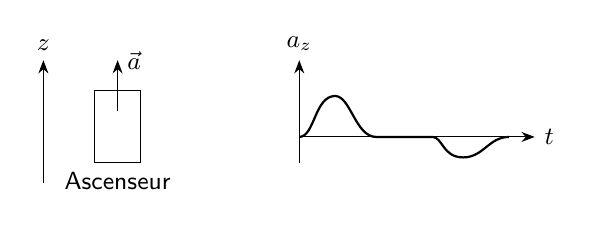
\begin{tikzpicture}[scale=.65]
\draw[->] (-1,-.4)--(-1,2) node[above]{$z$};\draw (0,0) rectangle(.9,1.4);\draw[->] (.45,1)--(.45,2) node[right]{$\vec a$};\node[below] at (.45,0){Ascenseur};
\begin{scope}[shift={(4,.5)}]\draw[->] (0,0)--(4.6,0) node[right]{$t$};\draw[->] (0,-.5)--(0,1.5) node[above]{$a_z$};\draw[thick] (0,0)..controls (.3,0) and (.3,.8)..(.7,.8)..controls (1,.8) and (1.1,0)..(1.5,0)--(2.6,0)..controls (2.8,0) and (2.8,-.4)..(3.2,-.4)..controls (3.6,-.4) and (3.7,0)..(4.1,0);\end{scope}
\end{tikzpicture}\end{center}
Pendant les phases d'accélération, il faut ajouter les forces d'inertie.
\begin{center}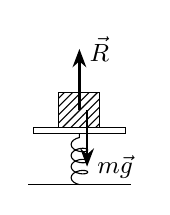
\begin{tikzpicture}[scale=.65]
\draw (-1,-1)--(1,-1);\draw[decorate,decoration={coil,segment length=4pt,amplitude=3pt}] (0,-1)--(0,0);\draw (-.9,0) rectangle(.9,.12);\draw[pattern=north east lines] (-.4,.12) rectangle(.4,.8);\draw[->,thick] (0,.45)--(0,1.65) node[right]{$\vec R$};\draw[->,thick] (.15,.45)--(.15,-.65) node[right]{$m\vec g$};
\end{tikzpicture}\end{center}
\textbf{2) Un mouvement rectiligne non uniforme}
\begin{center}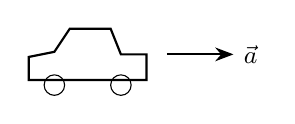
\begin{tikzpicture}[scale=.65]
\draw[thick] (0,0)--(0,.45)--(.5,.55)--(.8,1)--(1.6,1)--(1.8,.5)--(2.3,.5)--(2.3,0)--cycle;\draw (.5,-.1) circle(.2);\draw (1.8,-.1) circle(.2);\draw[->,thick] (2.7,.5)--(4,.5) node[right]{$\vec a$};
\end{tikzpicture}\end{center}
\textbf{3) Un virage}
\begin{center}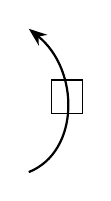
\begin{tikzpicture}[scale=.65]\draw[->,thick] (0,-1)..controls (1,-.6) and (1,1)..(0,1.8);\draw (.45,.15) rectangle(1.05,.8);\end{tikzpicture}\end{center}
\textbf{4) Un manège}
\begin{center}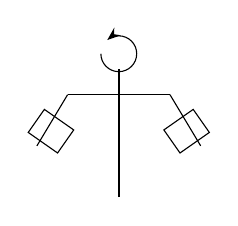
\begin{tikzpicture}[scale=.65]\draw[thick] (0,-1)--(0,1.5);\draw (-1,1)--(1,1);\draw (-1,1)--(-1.6,0);\draw (1,1)--(1.6,0);\draw[rotate=-35] (-1.6,-.8) rectangle(-.9,-.25);\draw[rotate=35] (.9,-.8) rectangle(1.6,-.25);\draw[->] (-.35,1.8) arc(180:490:.35);\end{tikzpicture}\end{center}
\end{exemple}
\section{La loi de la quantité de mouvement et les forces d'inertie}
\subsection{Le principe fondamental}
\begin{center}\frames{1}\end{center}
$\Rg$ est galiléen. Le principe fondamental de la dynamique donne :
\[m\ag(M)=\vec F,\qquad m\bigl(\ap(M)+\ae(M)+\ac(M)\bigr)=\vec F.\]
\begin{cadre}\[m\ap(M)=\vec F-m\ae(M)-m\ac(M).\]\end{cadre}
\subsection{Les forces d'inertie}
\subsubsection{Quelques généralités}
\[\Fie=-m\ae(M)\quad\text{(force d'inertie d'entraînement)},\]
\[\Fic=-m\ac(M)\quad\text{(force d'inertie de Coriolis)}.\]
\titr{Principe fondamental de la dynamique}
\begin{cadre}[etoiles={\etoiles{5}}]\[m\ap(M)=\vec F+\underbrace{\Fie+\Fic}_{\text{forces d'inertie ou pseudo-forces}}.\]\end{cadre}
% Source : pages 5-6.
\begin{itemize}
\item Ce ne sont pas de vraies forces : elles dépendent du référentiel.
\item Elles traduisent des effets d'inertie dans les référentiels non galiléens.
\item Dans le cas d'une translation rectiligne uniforme par rapport à $\Rg$ :
\[\ac=\vec0,\quad\ae(M)=\ag(O')=\vec0,\qquad\Fic=\vec0,\quad\Fie=\vec0.\]
D'où $m\ap=\vec F$. On retrouve que $\R'$ est galiléen.
\end{itemize}
\[\Fic=-m\ac(M).\]
\begin{cadre}[etoiles={\etoiles{5}}]\[\Fic=-2m\Om\wedge\vp(M).\]\end{cadre}
Cette expression est du même type que celle de la force de Lorentz magnétique.
\begin{cadre}[etoiles={\etoiles{4}}]
La force de Coriolis est toujours perpendiculaire à $\vp(M)$ : c'est une force déviatrice.
\end{cadre}
\[\pow_{\R'}(\Fic)=0.\]
Elle ne travaille pas.
\begin{cadre}[etoiles={\etoiles{5}}]
\[\begin{aligned}\Fic=\vec0\quad&\longrightarrow\quad\Om=\vec0 : \R'\text{ en translation dans }\Rg,\\&\longrightarrow\quad\vp(M)=\vec0 : \text{absence de mouvement relatif}.\end{aligned}\]
\end{cadre}
\subsubsection{Cas d'un référentiel $\R'$ en translation par rapport à $\R$}
\begin{cadre}[etoiles={\etoiles{4}}]\[\Fic=\vec0,\qquad\Fie=-m\ae(M)=-m\vec{a}_{\R}(O').\]\end{cadre}
\begin{exemple}[breakable]
\titr{Exemple : ascenseur}
$\R'$ est le référentiel de l'ascenseur, en translation rectiligne non uniforme.
\begin{center}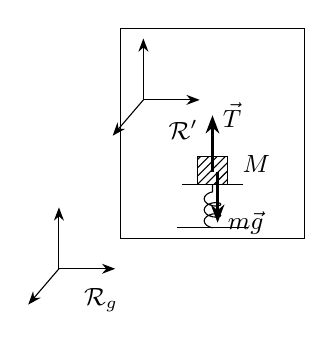
\begin{tikzpicture}[scale=.65]
\draw (-.8,-.8) rectangle(2.8,3.3);\begin{scope}[shift={(-.35,1.9)}]\rep{\R'}\end{scope}
\draw (.3,-.6)--(1.7,-.6);\draw[decorate,decoration={coil,segment length=4pt,amplitude=3pt}] (1,-.6)--(1,.25);\draw (.4,.25)--(1.6,.25);\draw[pattern=north east lines] (.7,.25) rectangle(1.3,.8);\node[right] at (1.4,.65){$M$};\draw[->,thick] (1,.5)--(1,1.6) node[right]{$\vec T$};\draw[->,thick] (1.1,.5)--(1.1,-.5) node[right]{$m\vec g$};
\begin{scope}[shift={(-2,-1.4)}]\rep{\Rg}\end{scope}
\end{tikzpicture}\end{center}
Le système est le poids $M$. Le bilan des forces comprend $m\vec g$ et $\vec T$, réaction du support, égale à la force de tension du ressort.
\[\Fie=-ma\vec u_z,\]
où $a$ est l'accélération de l'ascenseur.
\begin{center}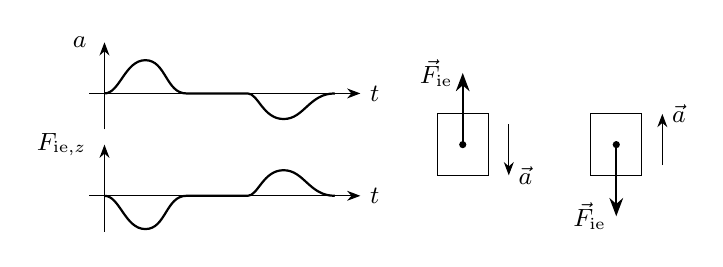
\begin{tikzpicture}[scale=.65]
\foreach \y/\lab/\sg in {0/a/1,-2/{F_{\mathrm{ie},z}}/-1}{\begin{scope}[shift={(0,\y)}]\draw[->] (0,-.7)--(0,1) node[left,xshift=-3pt]{$\lab$};\draw[->] (-.3,0)--(5,0) node[right]{$t$};\draw[thick] (0,0)..controls (.3,0) and (.4,\sg*.65)..(.8,\sg*.65)..controls (1.2,\sg*.65) and (1.2,0)..(1.6,0)--(2.8,0)..controls (3,0) and (3.1,-\sg*.5)..(3.5,-\sg*.5)..controls (3.9,-\sg*.5) and (4,0)..(4.5,0);\end{scope}}
\begin{scope}[shift={(7,-1)}]\foreach \x/\sg in {0/1,3/-1}{\begin{scope}[shift={(\x,0)}]\draw (-.5,-.6) rectangle(.5,.6);\fill (0,0) circle(2pt);\draw[->,thick] (0,0)--(0,\sg*1.4) node[left]{$\Fie$};\draw[->] (.9,\sg*.4)--(.9,-\sg*.6) node[right]{$\vec a$};\end{scope}}\end{scope}
\end{tikzpicture}\end{center}
La réduction de masse lue est $\Delta m$.
\[\Delta m\,g=F_{\mathrm{ie}}=m|a|,\qquad |a|=\frac{\Delta m\,g}{m}=0{,}6\ \mathrm{m\,s^{-2}}.\]
\end{exemple}
\subsubsection{Cas d'un référentiel $\R'$ en rotation uniforme autour d'un axe fixe dans $\R$}
\begin{center}\rotationfig{0}\end{center}
\begin{cadre}\[\Fic=-2m\Omega_{\R'/\R}\wedge\vp(M).\]\end{cadre}
\[\Fie=-m\ae(M)=-m\bigl(-\Omega_{\R'/\R}^{2}\overrightarrow{HM}\bigr).\]
\begin{cadre}[etoiles={\etoiles{4}}]\[\Fie=m\Omega_{\R'/\R}^{2}\overrightarrow{HM}.\]\end{cadre}
C'est la force centrifuge. Elle est dirigée vers l'extérieur par rapport à l'axe.
\begin{itemize}\item Lorsque $\Omega_{\R'/\R}$ augmente, $F_{\mathrm{ie}}$ augmente.
\item Lorsque $\|\overrightarrow{HM}\|$ augmente, $F_{\mathrm{ie}}$ augmente.\end{itemize}
\begin{exemple}
\titr{Exemple : centrifuger de l'eau}
\begin{center}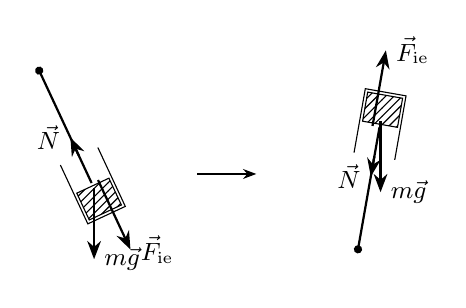
\begin{tikzpicture}[scale=.75]
\foreach \x/\ang in {0/25,5/170}{\begin{scope}[shift={(\x,0)}]\begin{scope}[rotate=\ang]\draw[thick] (0,1.6)--(0,0);\fill (0,1.6) circle(2pt);\draw (-.35,0)--(-.35,-1.1)--(.35,-1.1)--(.35,0);\draw[pattern=north east lines] (-.3,-.55) rectangle(.3,-1.05);\draw[->,thick] (0,-.5)--(0,.35) node[left]{$\vec N$};\draw[->,thick] (.12,-.5)--(.12,-1.8) node[right]{$\Fie$};\coordinate (W) at (0,-.6);\end{scope}\draw[->,thick] (W)--++(0,-1.2) node[right]{$m\vec g$};\end{scope}}
\draw[->] (2,-.3)--(3,-.3);
\end{tikzpicture}\end{center}
La force d'inertie est proportionnelle à $m$.
\end{exemple}
\subsection{Cas des systèmes}
\begin{center}\frames{2}\end{center}
\titr{Premier point de vue}
Pour tout $i$, le principe fondamental de la dynamique donne :
\[m_i\ap(P_i)=\vec F_i+\Fie(P_i)+\Fic(P_i).\]
On somme sur tous les points :
\[\underbrace{\sum_i m_i\ap(P_i)}_{=\mt\ap(G)}=
\underbrace{\sum_i\vec F_i}_{=\vec F_{\mathrm{ext}}+\underbrace{\vec F_{\mathrm{int}}}_{=\vec0}}
+\sum_i-m_i\ae(P_i)+\sum_i-m_i\ac(P_i).\]
\begin{cadre}\[\mt\ap=\vec F_{\mathrm{ext}}+\Fie+\Fic.\]\end{cadre}
$\Fie$ et $\Fic$ sont les résultantes des forces d'inertie appliquées à tous les points :
\[\Fie=\sum_i-m_i\ae(P_i),\qquad\Fic=\sum_i-m_i\ac(P_i).\]
\titr{Deuxième point de vue}
Le théorème de la quantité de mouvement dans $\Rg$ pour $\Sigma$ s'écrit :
\[\mt\underbrace{\ag(G)}_{=\ap(G)+\ae(G)+\ac(G)}=\vec F_{\mathrm{ext}}.\]
\begin{cadre}\[\mt\ap(G)=\vec F_{\mathrm{ext}}-\mt\ae(G)-\mt\ac(G).\]\end{cadre}
\titr{Lien entre les deux}
\begin{align*}
\sum_i\bigl(-m_i\ac(P_i)\bigr)&=\sum_i-2m_i\Om\wedge\vp(P_i)\\
&=-2\Om\wedge\sum_i m_i\vp(P_i)\\
&=-2\Om\wedge\mt\vp(G)\\
&=-\mt\bigl(2\Om\wedge\vp(G)\bigr).
\end{align*}
\begin{cadre}\[\Fic=-\mt\ac(G).\]\end{cadre}
D'où :
\begin{cadre}\[\Fie=\sum_i\bigl(-m_i\ae(P_i)\bigr)=-\mt\ae(G).\]\end{cadre}
\titr{Théorème de la quantité de mouvement dans $\R'$}
\begin{cadre}[etoiles={\etoiles{5}}]\[\mt\ap(G)=\vec F_{\mathrm{ext}}+\Fie+\Fic,\]
\[\text{avec}\qquad\Fie=-\mt\ae(G),\qquad\Fic=-\mt\ac(G).\]\end{cadre}
Dans $\R'$ non galiléen, le théorème de la quantité de mouvement appliqué à un système reste valable à condition d'ajouter aux forces extérieures la résultante des forces d'entraînement et des forces de Coriolis.
% Source : pages 11-13.
\section{Théorème du moment cinétique}
\subsection{Théorème du moment cinétique pour un point matériel}
Dans $\Rg$, avec $O$ fixe dans $\Rg$ :
\[\D{\vec L_{O/\Rg}(M)}{\Rg}=\overrightarrow{OM}\wedge\vec F.\]
Dans $\R'$, par définition du moment cinétique :
\[\vec L_{O'/\R'}(M)=\overrightarrow{O'M}\wedge m\vp(M).\]
\begin{align*}
\D{\vec L_{O'/\R'}(M)}{\R'}
&=\underbrace{\underbrace{\D{\overrightarrow{O'M}}{\R'}}_{=\vp(M)}\wedge m\vp(M)}_{=\vec0}
+\overrightarrow{O'M}\wedge m\underbrace{\D{\vp(M)}{\R'}}_{=\ap(M)}\\
&=\overrightarrow{O'M}\wedge\underbrace{m\ap(M)}_{\substack{\text{terme du théorème}\\\text{de la quantité de mouvement}}}.
\end{align*}
\[\D{\vec L_{O'/\R'}(M)}{\R'}=\overrightarrow{O'M}\wedge\bigl[\vec F+\Fie+\Fic\bigr].\]
\titr{Théorème du moment cinétique dans $\R'$ avec $O'$ fixe dans $\R'$}
\begin{cadre}[etoiles={\etoiles{5}}]
\[\D{\vec L_{O'/\R'}(M)}{\R'}=\mom{O'}(\vec F)+\mom{O'}(\Fie)+\mom{O'}(\Fic).\]
\end{cadre}
Le théorème du moment cinétique reste valable dans $\R'$ non galiléen pour un point matériel, par rapport à un point fixe, à condition d'ajouter les moments des forces d'inertie et de Coriolis.
De la même manière, par rapport à un axe $\Delta$ fixe :
\begin{cadre}[etoiles={\etoiles{5}}]
\[\D{L_{\Delta/\R'}(M)}{\R'}=\mathcal M_\Delta(\vec F)+\mathcal M_\Delta(\Fie)+\mathcal M_\Delta(\Fic).\]
\end{cadre}
\subsection{Cas des systèmes}
\begin{center}\frames{2}\end{center}
\[\D{\vec L_{O'/\R'}(P_i)}{\R'}=
\mom{O'}(\vec F_{\to P_i})+\mom{O'}\bigl(\Fie(P_i)\bigr)+\mom{O'}\bigl(\Fic(P_i)\bigr).\]
En sommant sur tous les points :
\[\D{\vec L_{O'/\R'}(\Sigma)}{\R'}=\mom{O',\mathrm{ext}}+\underbrace{\mom{O',\mathrm{int}}}_{=\vec0}+\mom{O',\mathrm{ie}}+\mom{O',\mathrm{ic}}.\]
\begin{cadre}[etoiles={\etoiles{4}}]
\[\D{\vec L_{O'/\R'}(\Sigma)}{\R'}=\mom{O',\mathrm{ext}}+\mom{O',\mathrm{ie}}+\mom{O',\mathrm{ic}}.\]
\end{cadre}
Pour un axe $\Delta$ fixe :
\begin{cadre}[etoiles={\etoiles{6}}]
\[\D{L_{\Delta/\R'}(\Sigma)}{\R'}=\mathcal M_{\Delta,\mathrm{ext}}+\mathcal M_{\Delta,\mathrm{ie}}+\mathcal M_{\Delta,\mathrm{ic}}.\]
\end{cadre}
% Source : pages 14-15.
\[\mom{O',\mathrm{ie}}=\sum_i\overrightarrow{O'P_i}\wedge\bigl(-m_i\ae(P_i)\bigr),\]
\[\mom{O',\mathrm{ic}}=\sum_i\overrightarrow{O'P_i}\wedge\bigl(-m_i\ac(P_i)\bigr).\]
Ce sont les moments résultants des forces d'inertie. Aucune simplification n'est possible en général : le moment résultant est différent du moment de la force résultante.
\titr{Cas particulier : $\R'$ en translation par rapport à $\Rg$}
\[\ae(P_i)=\ag(O').\]
L'accélération d'entraînement a la même valeur pour tous les points. Comme pour le poids, on peut considérer la résultante de tous les $\ae$ en $G$.
\[\Fie=-\mt\ae(G)=-\mt\ag(O').\]
\begin{align*}
\mom{O',\mathrm{ie}}&=\sum_i\overrightarrow{O'P_i}\wedge\bigl(-m_i\ag(O')\bigr)\\
&=-\left(\sum_i m_i\overrightarrow{O'P_i}\right)\wedge\ag(O')\\
&=\mt\overrightarrow{O'G}\wedge\bigl(-\ag(O')\bigr)\\
&=\overrightarrow{O'G}\wedge\Fie.
\end{align*}
Donc, dans le cas d'une translation :
\begin{cadre}[etoiles={\etoiles{2}}]
\[\begin{aligned}\Fic&=\vec0,&\mom{O',\mathrm{ic}}&=\vec0,\\
\Fie&=-\mt\ag(O'),&\mom{O',\mathrm{ie}}&=\overrightarrow{O'G}\wedge\Fie.
\end{aligned}\]
\end{cadre}
Dans le cas d'une translation de $\R'$ par rapport à $\Rg$, les forces d'inertie d'entraînement se comportent comme une seule force résultante appliquée en $G$.
\Needspace{45mm}\begin{exemple}[breakable]
\titr{Exemple : référentiel barycentrique}
\begin{center}\baryfig{1}\end{center}
\[\bigl\{\Fie(P_i)\bigr\}\quad\Longleftrightarrow\quad\Fie\text{ en }G.\]
On applique le théorème du moment cinétique à $\Sigma$ dans $\R^*$ par rapport à $G$, point fixe de $\R^*$ :
\[\D{\vec L_{G/\R^*}(\Sigma)}{\R^*}=\mom{G}^{\mathrm{ext}}+\underbrace{\vec0}_{\Fic=\vec0}+\underbrace{\overrightarrow{GG}\wedge\Fie}_{=\vec0}.\]
Dans le cas d'un référentiel barycentrique, les forces d'inertie n'interviennent pas dans le théorème du moment cinétique.
\begin{center}\baryfig{0}\end{center}
Le théorème de la quantité de mouvement dans $\Rg$, en négligeant les frottements, donne :
\[\mt\ag(G)=\mt\vec g.\]
Le mouvement est parabolique.
Le théorème du moment cinétique dans $\R^*$ par rapport à $G$ donne :
\[\D{\vec L_{G/\R^*}(S)}{\R^*}=\underbrace{\overrightarrow{GG}\wedge\mt\vec g}_{\text{moment du poids}}+\underbrace{\vec0}_{\mathcal M_{\mathrm{ic}}}+\underbrace{\vec0}_{\mathcal M_{\mathrm{ie}}}=\vec0.\]
\[\vec L_{G/\R^*}(S)=\overrightarrow{\cste}.\]
\end{exemple}
% Source : pages 16-18.
\section{Théorèmes énergétiques}
\subsection{Théorèmes énergétiques pour un point matériel}
\begin{center}\frames{1}\end{center}
Le principe fondamental de la dynamique appliqué à $M$ dans $\R'$ s'écrit :
\[m\ap(M)=\vec F+\Fie+\Fic.\]
\[m\D{\vp(M)}{\R'}\cdot\vp(M)=\vec F\cdot\vp(M)+\Fie\cdot\vp(M)+\Fic\cdot\vp(M).\]
\begin{cadre}[etoiles={\etoiles{6}}]
\[\D{E_{c/\R'}(M)}{\R'}=\pow_{\R'}(\vec F)+\pow_{\R'}(\Fie)+\underbrace{\pow_{\R'}(\Fic)}_{=0}.\]
\end{cadre}
Le théorème de l'énergie cinétique dans $\R'$ non galiléen s'écrit de la même manière que dans un référentiel galiléen, à condition de considérer les puissances des forces d'inertie.
De plus, $\pow_{\R'}(\Fic)=0$, car $\Fic\perp\vp$.
\titr{Théorème de l'énergie cinétique}
\begin{cadre}\[\Delta E_{c/\R'}(M)=W_{\R'}(\vec F)+W_{\R'}(\Fie).\]\end{cadre}
\subsection{Force d'inertie d'entraînement et énergie potentielle}
A priori, il n'y a pas de résultat général.
\titr{Premier cas particulier}
$\R'$ est en translation rectiligne uniformément accélérée par rapport à $\Rg$.
\begin{center}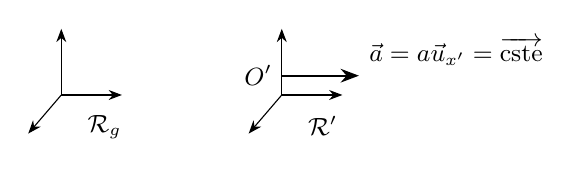
\begin{tikzpicture}[scale=.7]
\rep{\Rg}\begin{scope}[shift={(4,0)}]\rep{\R'}\node[above left] at (0,0){$O'$};\draw[->,thick] (0,.35)--(1.4,.35) node[above right]{$\vec a=a\vec u_{x'}=\overrightarrow{\cste}$};\end{scope}
\end{tikzpicture}\end{center}
\[\Fie=-m\ag(O')=-ma\vec u_{x'}=-\grad\Ep.\]
\begin{cadre}[etoiles={\etoiles{3}}]\[\Ep=max'+\cste.\]\end{cadre}
\titr{Deuxième cas particulier}
$\R'$ est en rotation uniforme autour d'un axe fixe $\Delta$ dans $\Rg$.
\begin{center}\rotationfig{1}\end{center}
\[\Fie=m\Omega_{\R'/\Rg}^{2}\overrightarrow{HM}.\]
Dans la base cylindrique d'axe $\Delta$ :
\[m\Omega_{\R'/\Rg}^{2}r\vec u_r=-\grad\Ep,\qquad
\grad=\vec u_r\frac{\partial}{\partial r}+\vec u_\theta\frac1r\frac{\partial}{\partial\theta}+\vec u_z\frac{\partial}{\partial z}.\]
\begin{cadre}[etoiles={\etoiles{5}}]\[\Ep=-\frac12m\Omega_{\R'/\Rg}^{2}r^2+\cste.\]\end{cadre}
Le signe est négatif : l'énergie décroît lorsque $r$ augmente, car la force centrifuge pousse vers l'extérieur.
% Source : page 20.
\Needspace{40mm}\titr{Théorème de l'énergie mécanique}
\[\D{E_{m/\R'}(M)}{\R'}=\pow_{\R'}(\text{forces non conservatives}).\]
Les forces considérées sont les vraies forces et, selon sa nature, $\Fie$.
\[E_{m/\R'}(M)=E_{c/\R'}(M)+\underbrace{E_{p/\R'}(M)}_{\text{vraies forces}}\ \bigl(+E_{p\mathrm{ie}/\R'}(M)\bigr).\]
\subsection{Cas des systèmes}
\begin{center}\frames{2}\end{center}
Pour $P_i$ :
\[\D{E_{c/\R'}(P_i)}{\R'}=\pow_{\R'}(\vec F_{\to P_i})+\pow_{\R'}(\Fie).\]
En sommant sur tous les points $P_i$ :
\begin{cadre}[etoiles={\etoiles{4}}]\[\D{E_{c/\R'}(\Sigma)}{\R'}=\pow_{\R'}^{\mathrm{ext}}+\pow_{\R'}^{\mathrm{int}}+\pow_{\R'}^{\mathrm{ie}}.\]\end{cadre}
La puissance intérieure $\pow_{\R'}^{\mathrm{int}}$ est indépendante de $\R'$. Elle est nulle si le système est indéformable.
\begin{cadre}\[\Delta E_{c/\R'}(\Sigma)=W_{\mathrm{ext}}+W_{\mathrm{int}}+W_{\R',\mathrm{ie}}.\]\end{cadre}
La puissance résultante des forces d'inertie d'entraînement est :
\[\pow_{\R'}^{\mathrm{ie}}=\sum_i-m_i\ae(P_i)\cdot\vp(P_i).\]
Il n'y a pas de simplification générale.
\[\D{E_{m/\R'}(\Sigma)}{\R'}=\pow_{\R'}(\text{forces non conservatives}).\]
Il s'agit des forces extérieures, intérieures et d'inertie d'entraînement.
\[E_{m/\R'}(\Sigma)=E_{c/\R'}(\Sigma)+E_{p/\R'}^{\mathrm{ext}}(\Sigma)+E_{p/\R'}^{\mathrm{int}}(\Sigma)+E_p^{\mathrm{ie}}(\Sigma).\]
\end{document}